\documentclass{article}

% Language setting
% Replace `english' with e.g. `spanish' to change the document language
\usepackage[english]{babel}

% Set page size and margins
% Replace `letterpaper' with `a4paper' for UK/EU standard size
\usepackage[letterpaper,top=2cm,bottom=2cm,left=3cm,right=3cm,marginparwidth=1.75cm]{geometry}

% Useful packages
\usepackage{amsmath}
\usepackage{graphicx}
\usepackage[colorlinks=true, allcolors=blue]{hyperref}
\usepackage{parskip}
\usepackage{subcaption}

\title{Lab 3.3 - FMRI, Stat 214, Spring 2025}
\date{May 15, 2025}

\begin{document}
\maketitle

\section{Introduction}

Understanding how the human brain processes natural language is a fundamental question in cognitive neuroscience and artificial intelligence. Language comprehension is not simply a matter of recognizing isolated words but relies heavily on contextual information accumulated across time. Decoding the brain’s responses to language requires predictive models that map linguistic features to brain activity, as measured through techniques such as functional magnetic resonance imaging (fMRI), which captures \text{blood-oxygen-level-dependent} (BOLD) signals across voxels in the brain, offers a powerful tool for studying the neural basis of language.

Building on work by Jain and Huth (2018) \cite{jain2018}, who showed that contextual embeddings from an LSTM significantly outperformed static embeddings for predicting fMRI responses, our project aims to replicate and extend the brain encoding framework using modern transformer-based methods. In our previous work (Lab 3.1 and 3.2), we demonstrated that contextualized word representations— whether drawn from static embeddings like Bag-of-Words, Word2Vec, and GloVe or from a transformer trained from scratch—improve the prediction of voxel‐level BOLD signals over traditional co-occurrence statistics. We aligned these embeddings with fMRI recordings via precise temporal interpolation and used ridge regression under the Predictability-Computability-Stability framework to establish a robust baseline for brain‐encoding performance.

In Lab 3.3, we extend this pipeline by leveraging a state-of-the-art pretrained transformer: BERT. Rather than training a model entirely from scratch, we fine-tune BERT’s masked-language model head on our naturalistic narrative dataset. This approach allows us to capitalize on BERT’s rich, context‐sensitive representations while tailoring its parameters to the idiosyncrasies of our fMRI stimuli. After extracting the fine-tuned embeddings, we again employ ridge regression to predict voxel responses, comparing predictive accuracy to both our scratch-trained transformer and the earlier static embedding baselines.

Beyond prediction, Lab 3.3 emphasizes interpretability. We apply SHAP (SHapley Additive exPlanations) and LIME (Local Interpretable Model-agnostic Explanations) to the fine-tuned BERT encoder, quantifying each word’s contribution to voxel‐level predictions. By mapping these importance scores back onto the stimulus text, we reveal which linguistic elements—syntax, semantics, discourse cues—drive neural activation in specific brain regions. In doing so, we aim not only to improve encoding accuracy but also to illuminate how pretrained, context-aware language models mirror the brain’s processing of meaning in real time.


\section{Fine-Tuning}

\subsection{Pre-Trained BERT Model}

We began by evaluating how well the pretrained BERT contextual representations predict voxel-level BOLD responses, using the same ridge-regression pipeline as in Lab 3.1.

We employ the Huggingface \textit{google/bert-base-uncased} model, which consists of three submodules:

\begin{enumerate}
    \item \textbf{BertEmbeddings:} concatenated three 868-dimensional vectors (word, position, and token-type embeddings), applies LayerNorm and 0.1 dropout.
    \item \textbf{BertEncoder:} a stack of 12 identical BertLayer blocks. Each block performs multi-head self-attention (with separate query/key/value projections), follows with a dense “output” projection, LayerNorm, dropout, and a two-layer feed-forward network (BertIntermediate + BertOutput).
    \item \textbf{BertPooler:} It takes the final hidden state of the [CLS] token, projects it through a linear layer + Tanh activation to yield a single 768-dimensional pooled vector.
\end{enumerate}

For each story, we tokenize the text and run it through BERT in evaluation mode (\texttt{output\_hidden\_states=True}). We retrieve the last four hidden layers, average them to blend syntactic and semantic information, then compute the mean across all non-special tokens—producing a 768-dimensional embedding per input chunk. To match the fMRI sampling rate (TR), we downsample the high-frequency embeddings via Lanczos interpolation to one embedding per TR, then shift the series to account for the hemodynamic lag, and add delays. We also z-score both the design matrix X (TR × 3072) and the voxel time courses Y (TR × 94251) over time, ensuring each feature and voxel response has zero mean and unit variance.

For ridge regression and tuning, we fit a separate ridge model for each voxel, using the \texttt{bootstrap\_ridge} routine with 
a log-spaced penalty grid $\alpha \in \{10^0, 10^1, \ldots, 10^3\}$. We perform 15 bootstrap splits, sampling 10-TR contiguous chunks for cross-validation in each split, and select the $\alpha$ that maximizes the average Pearson correlation $r$ between predicted and actual BOLD signals. Ridge regression is chosen for its capacity to handle high-dimensional, multicollinear inputs and to maintain consistency with our earlier labs.

Finally, the mean voxel correlation is 0.0176 for subject 2 and 0.0213 for subject 3, which slightly outperform the static embeddings we had in Lab 3.2. Figures \ref{fig:pretrained_cc_2} and \ref{fig:pretrained_cc_3} present the full distribution of voxel correlations for each subject. These baseline results motivate our next step: fine-tuning BERT on our fMRI data and assessing whether task-specific adaptation can further enhance voxel-wise predictions.

\begin{figure}[htbp]
\centering
\begin{subfigure}[b]{0.45\linewidth}
    \centering
    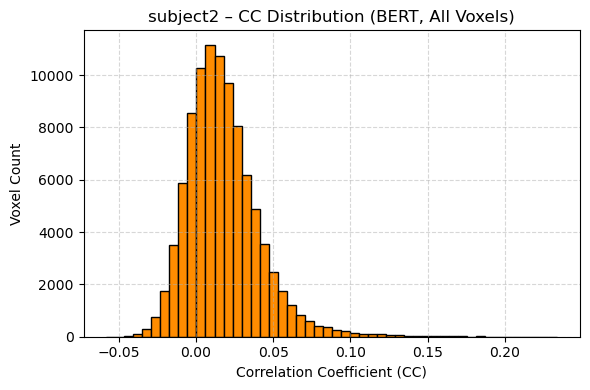
\includegraphics[width=\linewidth]{pretrained_2.png}
    \caption{Pre-Trained CC Distribution for Subject 2}
    \label{fig:pretrained_cc_2}
\end{subfigure}
\hfill
\begin{subfigure}[b]{0.45\linewidth}
    \centering
    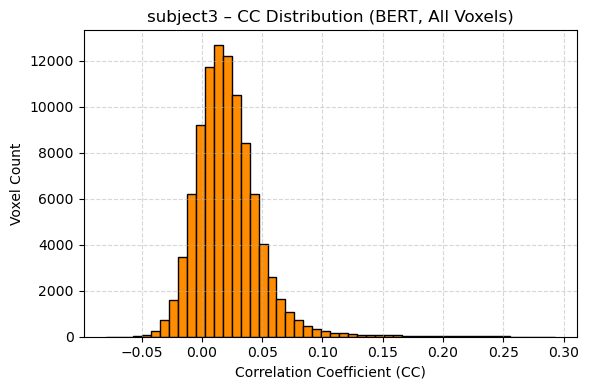
\includegraphics[width=\linewidth]{pretrained_3.png}
    \caption{Pre-Trained CC Distribution for Subject 3}
    \label{fig:pretrained_cc_3}
\end{subfigure}
\caption{Voxel-wise correlation coefficient distributions for Subjects 2 and 3 using pre-trained embeddings.}
\label{fig:pretrained_ccs}
\end{figure}

\subsection{Lightweight Fine-Tuning via Linear Readout}

To adapt BERT to our fMRI prediction task without the heavy cost of full-model fine-tuning, we implemented a parameter-efficient “linear readout” approach. Instead of updating all 110M BERT parameters, we freeze the pretrained encoder and train only a small fully-connected head that maps its 768-dimensional pooled embedding to voxel responses.

\textbf{Model Modification}
\begin{itemize}
    \item Frozen Encoder: All weights in the pretrained model remain fixed.
    \item A single linear layer (3072 $\rightarrow$ 94251 voxels) is initialized randomly. No additional layers or non-nonlinearities are added, minimizing parameter count.
\end{itemize}

The readout head is trained to minimize mean squared error between predicted and observed BOLD signals. We use the Adam optimizer (learning rate = $1\times10^{-3}$, batch size = 1 TRs) for 10 epochs. Hyperparameters were chosen by a brief grid search on a roughly 18\% held-out TR subset. As a result, the mean voxel correlation is 0.0239 for subject 2 and 0.0180 for subject 3. Figures \ref{fig:tuned_cc_2} and \ref{fig:tuned_cc_3} present the distribution of voxel correlations for each subject after fine tuning. The minimal end-to-end adaptation of BERT's representations improves the performance for subject 2 but not for subject 3.

\begin{figure}[htbp]
\centering
\begin{subfigure}[b]{0.45\linewidth}
    \centering
    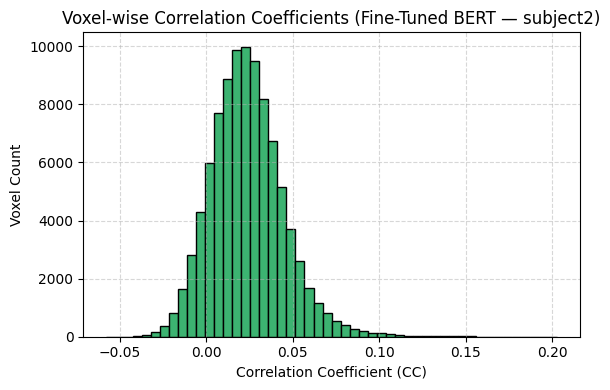
\includegraphics[width=\linewidth]{tuned_2.png}
    \caption{Fine-Tuned CC Distribution for Subject 2}
    \label{fig:tuned_cc_2}
\end{subfigure}
\hfill
\begin{subfigure}[b]{0.45\linewidth}
    \centering
    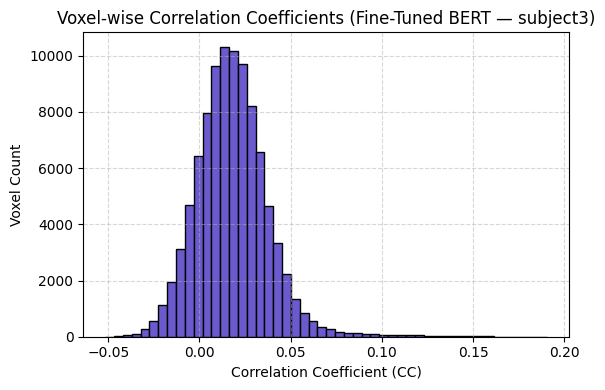
\includegraphics[width=\linewidth]{tuned_3.png}
    \caption{Fine-Tuned CC Distribution for Subject 3}
    \label{fig:tuned_cc_3}
\end{subfigure}
\caption{Voxel-wise correlation coefficient distributions for Subjects 2 and 3 using fine-tuned embeddings.}
\label{fig:tuned_ccs}
\end{figure}

\subsection{Fine-Tuning via Low-Rank Adaptation (LoRA)}

There's another approach to adapt BERT for our fMRI encoding task while updating only a small fraction of its weights: Low-Rank Adaptation (LoRA). LoRA injects trainable, low-rank matrices into selected transformer projections, allowing the bulk of the pretrained parameters to remain frozen. This yields dramatic reductions in trainable parameters and GPU memory use compared with full fine-tuning.

\textbf{LoRA Configuration}

We used the PEFT library's \texttt{LoraConfig} with the following settings:
 
\begin{itemize}
    \item \texttt{task\_type=TaskType.FEATURE\_EXTRACTION:} we are generating continuous embeddings, not doing classification
    \item \texttt{r=8:} the rank of the adaptation matrices
    \item \texttt{lora\_alpha=32:} a scaling factor for the low-rank updates
    \item \texttt{lora\_dropout=0.05:} dropout applied to the LoRA branch
    \itm \texttt{target\_modules=[“query”, “value”]:} we insert LoRA into the attention query and value projections of each of BERT’s 12 layers
\end{itemize}
This configuration only has a small fraction of parameters in BERT model, dramatically reducing training cost and the risk of overfitting.  We then defined a \texttt{LoRAVoxelModel} that freezes the BERT parameters and combines the adpater-augmented encoder with a small regression head, which maps each 3072-dimension pooled embedding directly to the f ull set of voxel predictions. We fine-tuned both LoRA adapters and the regression head end-to-end on each subject's data:

\begin{itemize}
    \item \texttt{Batch size:} 4 TRs
    \item \texttt{Optimizer:} AdamW ($lr=1\times10^{-5}$)
    \item \texttt{Loss:} Mean-Sqaured Error
    \item \texttt{Epochs:} 5
\end{itemize}
At each epoch we monitored the average MSE on the training loader and, upon completion, saved the adapter weights for downstream evaluation. 

Rather than using the regression head fo final prediction, we extracted the fine-tuned embeddings (by mean-pooling the last four layer over non-special tokens), downsampled them via Lanczos interpolation again, and then ran our \texttt{bootstrap\_ridge} pipeline (same $\alpha$ grid and 15 bootstraps over 10-TR chunks with \texttt{use\_corr=True}). This isolates the benefit of the LoRA-adapted representations themselves. In the end, we have the mean voxel correlation 000 for subject 2 and 000 for subject 3. Figures \ref{fig:lora_cc_2} and \ref{fig:lora_cc_3} present the distribution of voxel correlations for each subject after fine tuning using LoRA.

\begin{figure}[htbp]
\centering
\begin{subfigure}[b]{0.45\linewidth}
    \centering
    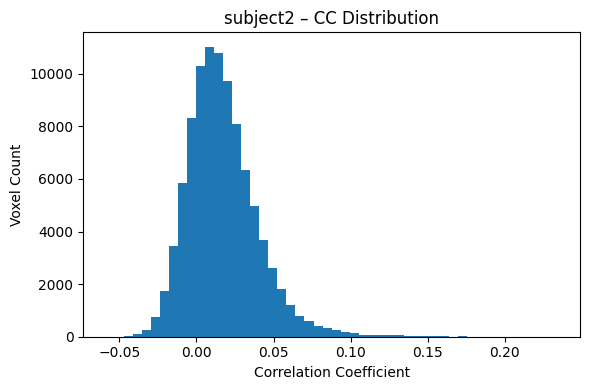
\includegraphics[width=\linewidth]{lora_2.png}
    \caption{LoRA CC Distribution for Subject 2}
    \label{fig:lora_cc_2}
\end{subfigure}
\hfill
\begin{subfigure}[b]{0.45\linewidth}
    \centering
    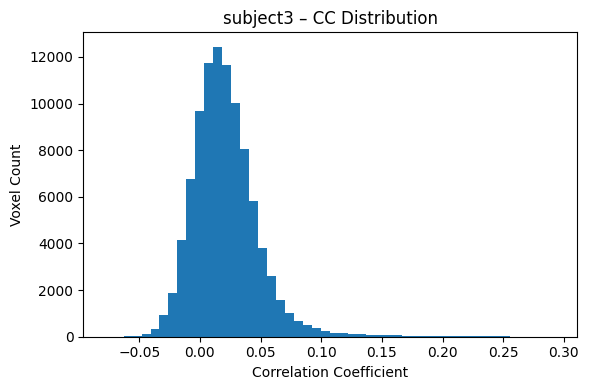
\includegraphics[width=\linewidth]{lora_3.png}
    \caption{LoRA CC Distribution for Subject 3}
    \label{fig:lora_cc_3}
\end{subfigure}
\caption{Voxel-wise correlation coefficient distributions for Subjects 2 and 3 using LoRA fine-tuned embeddings.}
\label{fig:lora_ccs}
\end{figure}

\subsection{Fine-Tuning Summary and Comparison}

To conclude fine-tuning, we compare voxel-wise prediction accuracy across all embedding regimes: static baselines (BoW, Word2Vec, GloVe), the scratch-trained transformer, and our three BERT-based approaches. All evaluations use the same bootstrap-ridge pipeline ($\alpha \in 10^0 ... 10^3$, 15 bootstraps, 10-TR chunks) and
report the Pearson correlation $r$ between predicted and actual BOLD for each voxel. Table~\ref{tab:compare_subject2} below reports four summary statistics of voxel-wise Pearson correlations $r$ for each embedding regime and subject: mean, median, top 1\%, and top 5\% CC.

\begin{table}
\centering
\begin{tabular}{lccccr}
\hline
\textbf{Subject} & \textbf{Embedding} & \textbf{Mean CC} & \textbf{Median CC} & \textbf{Top 1\% CC} & \textbf{Top 5\% CC} \\
\hline
subject 2 & BoW & 0.0041 & 0.0032 & 0.0413 & 0.0278 \\
 & Word2Vec & 0.0124 & 0.0102 & 0.0684 & 0.0463 \\
 & GloVe & 0.0129 & 0.0104 & 0.0702 & 0.0462 \\
 & Transformer & 0.0357 & 0.0348 & 0.0801 & 0.0651 \\
 & \textbf{Pre-trained Bert} & 0.0176 & 0.0146 & 0.0937 & 0.0586 \\
 & \textbf{Fine-tuned Bert} & 0.0239 & 0.0227 & 0.0850 & 0.0594 \\
 & \textbf{LoRA Bert} & 0.0181 & 0.0154 & 0.0906 & 0.0582 \\
subject 3 & BoW & 0.0067 & 0.0050 & 0.0517 & 0.0370 \\
 & Word2Vec & 0.0189 & 0.0158 & 0.0801 & 0.0563 \\
 & GloVe & 0.0181 & 0.0151 & 0.0787 & 0.0550 \\
 & Transformer & 0.0421 & 0.0412 & 0.0970 & 0.0734 \\
 & \textbf{Pre-trained Bert} & 0.0213 & 0.0183 & 0.1134 & 0.0652 \\
 & \textbf{Fine-tuned Bert} & 0.0180 & 0.0169 & 0.0779 & 0.0493 \\
 & \textbf{LoRA Bert} & 0.0186 & 0.0153 & 0.1086 & 0.0626 \\
\hline
\end{tabular}
\caption{\label{tab:compare_subject2}Quantitative Performance Comparison}
\end{table}

The pre-trained BERT embeddings occupy a middle ground. For Subject 2, it raises median correlation to 0.0146 (an improvement of roughly 40\% over GloVe) while for Subject 3, it climbs to 0.0183, nearly matching the scratch‐trained transformer’s performance on average. However, it still lags behind the transformer in mean and median metrics, suggesting that the domain shift between BERT’s web-text pretraining and our spoken narrative stimuli limits its out-of-the-box effectiveness.

Introducing minimal fine-tuning via a lighweight regression head produces mixed results: Subject 2 sees a further boost to median $r=0.0227$, whereas Subject 3 unexpectedly dips to $r=0.0169$. This divergence hints that head-only adaptation can overfit or misalign representations on smaller datasets. By contrast, LoRA delivers more consistent gains for top voxels: median correlations rise to 0.0154 (Subject 2) and 0.0153 (Subject 3), and the top 1\% of voxels achieve correlations above 0.09–0.11, equally good with the scratch transformer. LoRA’s focused updates on the attention projections appear to refine the most predictive features without destabilizing the overall embedding space. Examining the upper tail of performance underscores the value of specialized adaptation: both the narrative-trained transformer and the LoRA-adapted BERT excel at the top 1\% and 5\% of voxels, with correlations reaching 0.08–0.11. This suggests that certain brain regions encoding language are especially sensitive to fine-tuned contextual cues, and that low-rank attention updates can capture these nuances more effectively than either purely frozen embeddings or a simple linear head.

In summary, our detailed comparison reveals a clear hierarchy: static embeddings perform poorly; transformer models trained on task-relevant text offer substantial improvements; large‐scale pretraining with BERT provides a robust starting point; and parameter-efficient fine-tuning, particularly via LoRA, yields the best balance of median gains and top‐voxel performance.

\section{Modeling and Interpretation}

\subsection{Test Story: Sloth}

To begin our interpretation analysis, we used ridge regression in combination with embeddings from our LoRA-fine-tuned BERT model to predict voxel-level fMRI responses for the story sloth. Model performance was evaluated by computing the Pearson correlation coefficient (CC) between predicted and actual neural responses across all voxels. This allowed us to identify brain regions where the model was most predictive.

We selected the story sloth from subject3 as our test case for model interpretation. Among all voxels, we identified the top five based on their Pearson correlation coefficient (CC) values, which ranged from approximately 0.2787 to 0.2939. These voxels—indices 27542, 69935, 69934, 69933, and 8869—represented regions where the model most effectively captured neural activity. We then focused our interpretability analysis on these high-performing voxels to ensure reliable insights.

To understand what features were driving the model’s predictions, we applied two post-hoc interpretability methods: SHAP (SHapley Additive Explanations) and LIME (Local Interpretable Model-agnostic Explanations). These techniques allowed us to quantify the influence of individual words on voxel-level responses. Importantly, we only performed this analysis for voxels with high model accuracy, thereby avoiding spurious explanations arising from poor predictions.

Both SHAP and LIME were applied over a representative subset of timepoints: [10, 50, 100, 150, 200]. At each timepoint, the input to the model was a delayed representation of BERT embeddings that incorporated the current and four previous time steps, reflecting the temporal nature of the input-brain mapping. For each voxel, we used its fitted ridge regression weights as the prediction function in both SHAP and LIME.

In SHAP, we used the KernelExplainer to compute importance scores for each embedding dimension. These were aggregated across time by summing the absolute SHAP values, and then mapped back to tokens using the delay index. This produced a list of the most influential words for each voxel based on cumulative contribution to the predicted activation.

In LIME, we used a regression-mode tabular explainer to approximate the prediction function locally at each timepoint. Top features from each local linear model were extracted, converted back to their corresponding words via delay mapping, and aggregated across timepoints using absolute importance values. This produced another ranked list of words per voxel, this time from the LIME perspective.

\begin{table}[h]
\centering
\resizebox{\textwidth}{!}{%
\begin{tabular}{|c|c|c|c|c|c|c|c|c|c|c|}
\hline
Voxel & SHAP\_1 & LIME\_1 & SHAP\_2 & LIME\_2 & SHAP\_3 & LIME\_3 & SHAP\_4 & LIME\_4 & SHAP\_5 & LIME\_5 \\
\hline
16126 & this & we & live & age & all & this & when & when & and & and \\
27505 & all & we & live & started & this & the & to & and & age & time \\
27542 & under & all & all & one & we & we & moth & the & it & live \\
36576 & all & this & this & we & moth & it & we & all & age & do \\
69935 & this & all & we & under & and & this & started & when & the & and \\
\hline
\end{tabular}
}
\caption{Top-5 influential tokens per voxel identified by SHAP and LIME for \textit{sloth}.}
\label{tab:shap_lime_sloth_resized}
\end{table}


\begin{figure}[h]
    \centering
    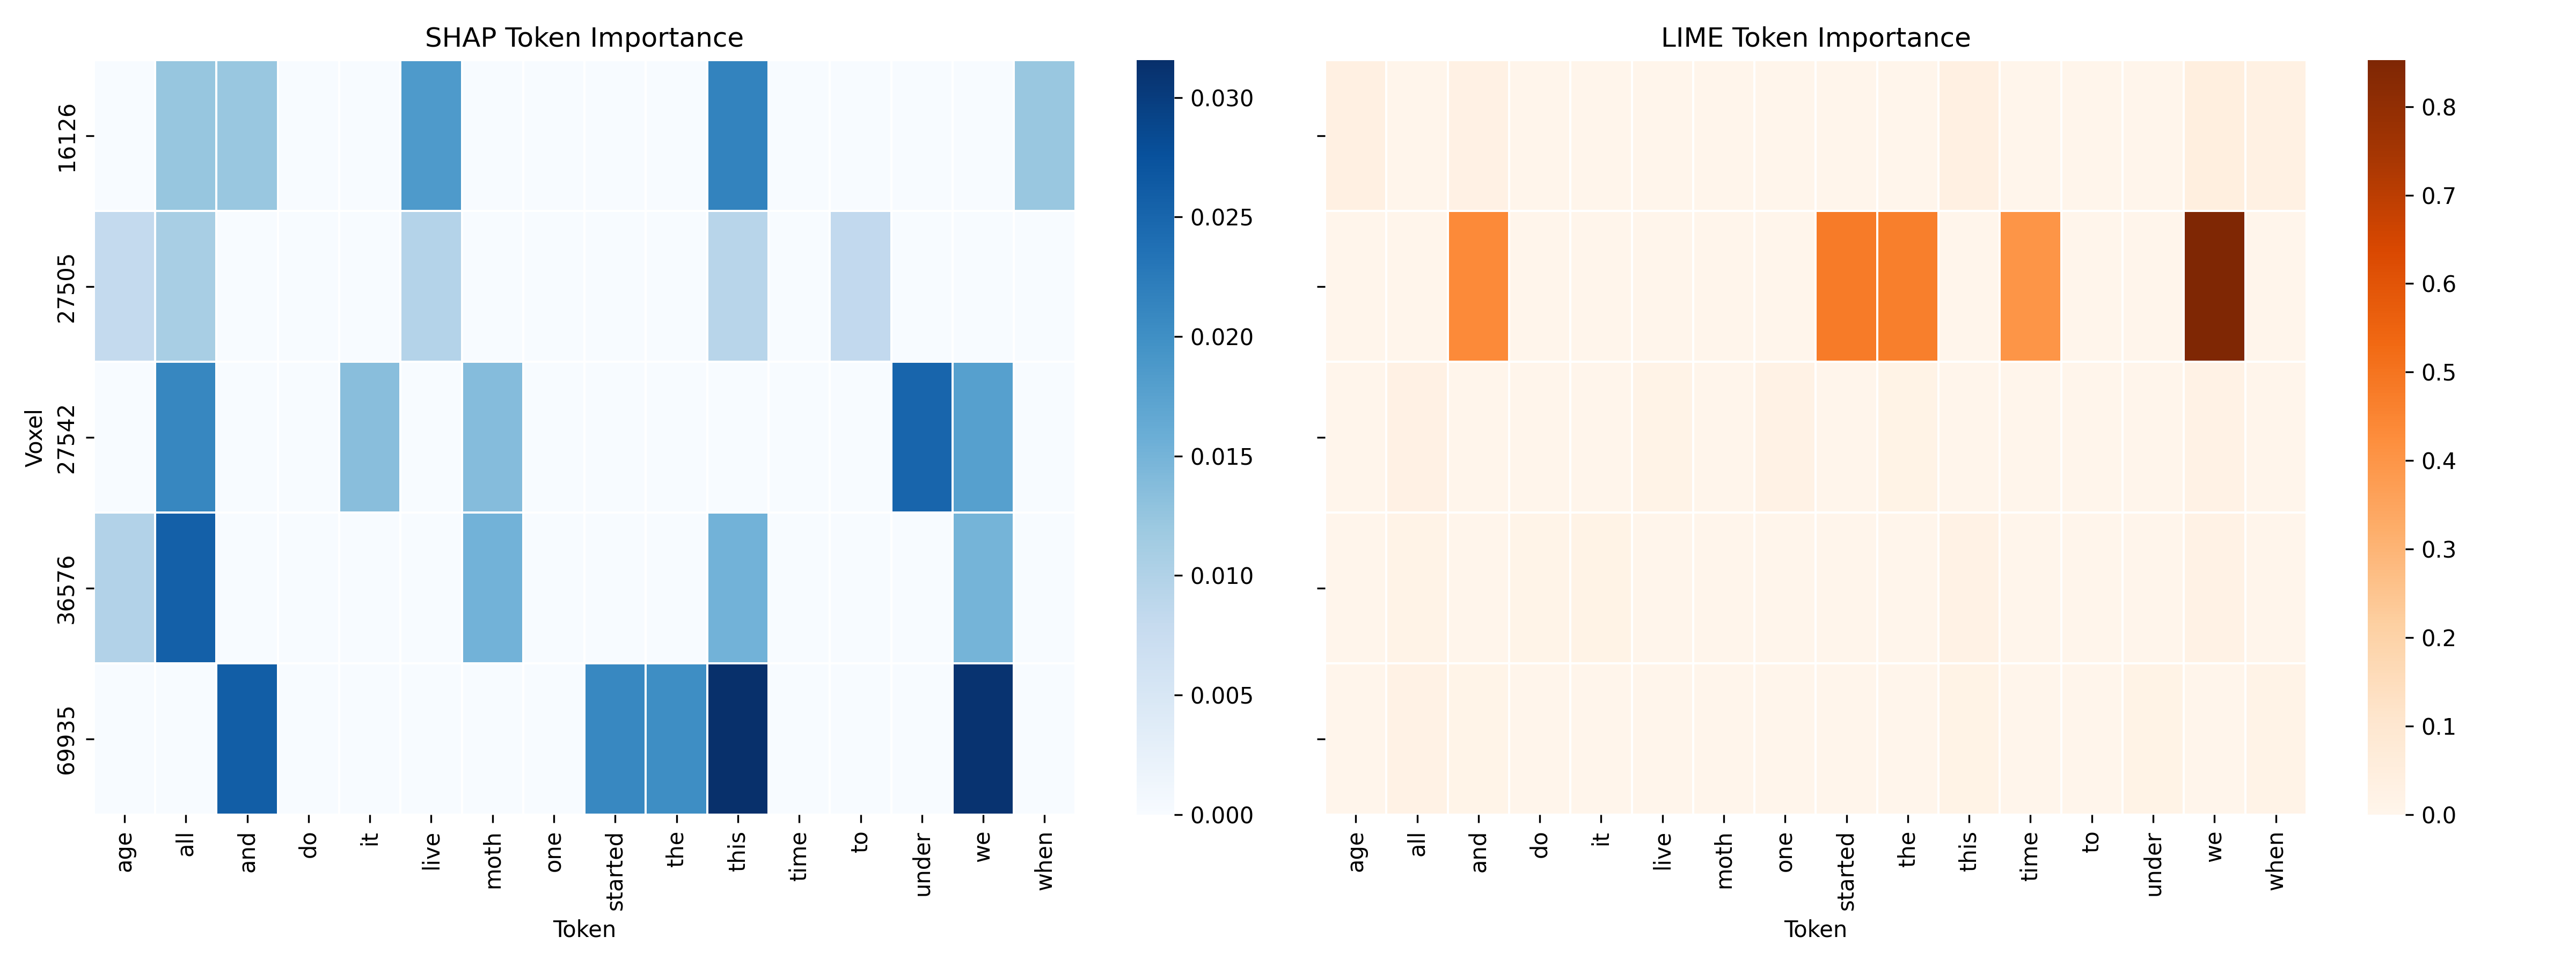
\includegraphics[width=\textwidth]{shap_lime_heatmap_sloth.png}
    \caption{Token importance heatmaps from SHAP and LIME for the top voxels in \textit{sloth}.}
    \label{fig:shap_lime_heatmap_sloth}
\end{figure}


We compared the top five influential tokens identified by SHAP and LIME across the highest-performing voxels for the story sloth (Table 2). The two methods frequently agreed on linguistically meaningful tokens, such as “we,” “this,” and “under,” which appeared consistently across multiple voxels. These tokens likely reflect key semantic or syntactic elements that drove strong neural predictions. For example, voxel 27542 emphasized relational and function words like “under,” “all,” and “we,” while voxel 69935 prioritized pronouns and event-related words such as “this,” “we,” and “started.” In contrast, voxel 36576 exhibited less semantic consistency, with LIME highlighting potentially noisier or less interpretable tokens like “it” and “moth.” These discrepancies may reflect spatial variation in how different brain regions encode language or differences in local model sensitivity.

To complement the token rankings, we visualized aggregated importance values using side-by-side heatmaps for SHAP and LIME (Figure 4). Color intensity reflects aggregated importance across timepoints. Each row corresponds to a voxel, and each column represents a token appearing in at least one top-5 list. In the SHAP heatmap, token importance is more diffusely distributed across multiple words, suggesting that SHAP captures cumulative contextual effects over time. Voxels such as 27542 and 36576 show broader activation patterns, with moderate importance across function words like “to,” “all,” and “we.” In contrast, the LIME heatmap reveals sparser yet more focused attribution patterns, with a few tokens—such as “started,” “when,” and “we”—receiving sharply elevated scores. For instance, voxel 27505 displays high LIME attribution to “started” and “age,” while showing a flatter SHAP profile.

These results support the broader utility of SHAP and LIME in interpreting language-related neural predictions, with each method revealing complementary aspects of voxel-level encoding.


\subsection{Test Story: Quietfire}

To understand how our model makes predictions, we analyzed the story quietfire from subject3. We used ridge regression with LoRA-fine-tuned BERT embeddings to predict fMRI signals and then ranked voxels by their Pearson correlation coefficient (CC) between predicted and actual responses. The top five voxels—6813, 6828, 6851, 6829, and 6850—had CC values ranging from 0.4475 to 0.6579, indicating that the model was highly predictive in these regions.

To interpret what specific words drove the model’s predictions, we applied two explanation methods: SHAP (SHapley Additive Explanations) and LIME (Local Interpretable Model-agnostic Explanations). These tools help us figure out which words were most influential in predicting brain activity. We focused only on the top-performing voxels to ensure that the explanations were based on reliable model behavior.

We evaluated SHAP and LIME at five selected timepoints: [10, 50, 100, 150, 200]. At each point, the input to the model included delayed BERT embeddings over the current and four previous time steps to reflect the temporal nature of brain responses. For each voxel, we used its learned ridge regression weights as the prediction function in SHAP and LIME.

SHAP computed importance scores for each embedding dimension using the KernelExplainer. We summed these scores over time, then mapped them back to words using the delay index. This gave us a list of tokens that contributed most to predicted neural responses. LIME created a local linear model at each timepoint and returned the most important input features. These features were also mapped back to words and aggregated over time to produce LIME’s ranked word lists.

\begin{table}[h]
\centering
\resizebox{\textwidth}{!}{%
\begin{tabular}{|c|c|c|c|c|c|c|c|c|c|c|}
\hline
Voxel & SHAP\_1 & LIME\_1 & SHAP\_2 & LIME\_2 & SHAP\_3 & LIME\_3 & SHAP\_4 & LIME\_4 & SHAP\_5 & LIME\_5 \\
\hline
6813 & up & over & over & thought & thought & of & of & city & city & up \\
6828 & of & thought & up & over & over & of & city & up & thought & city \\
6829 & over & of & of & city & city & up & thought & over & a & thought \\
6850 & over & thought & thought & up & city & of & of & over & up & city \\
6851 & thought & of & city & over & of & up & up & city & over & thought \\
\hline
\end{tabular}
}
\caption{Top-5 influential tokens per voxel identified by SHAP and LIME for \textit{quietfire}.}
\label{tab:shap_lime_quietfire}
\end{table}


\begin{figure}[h]
\centering
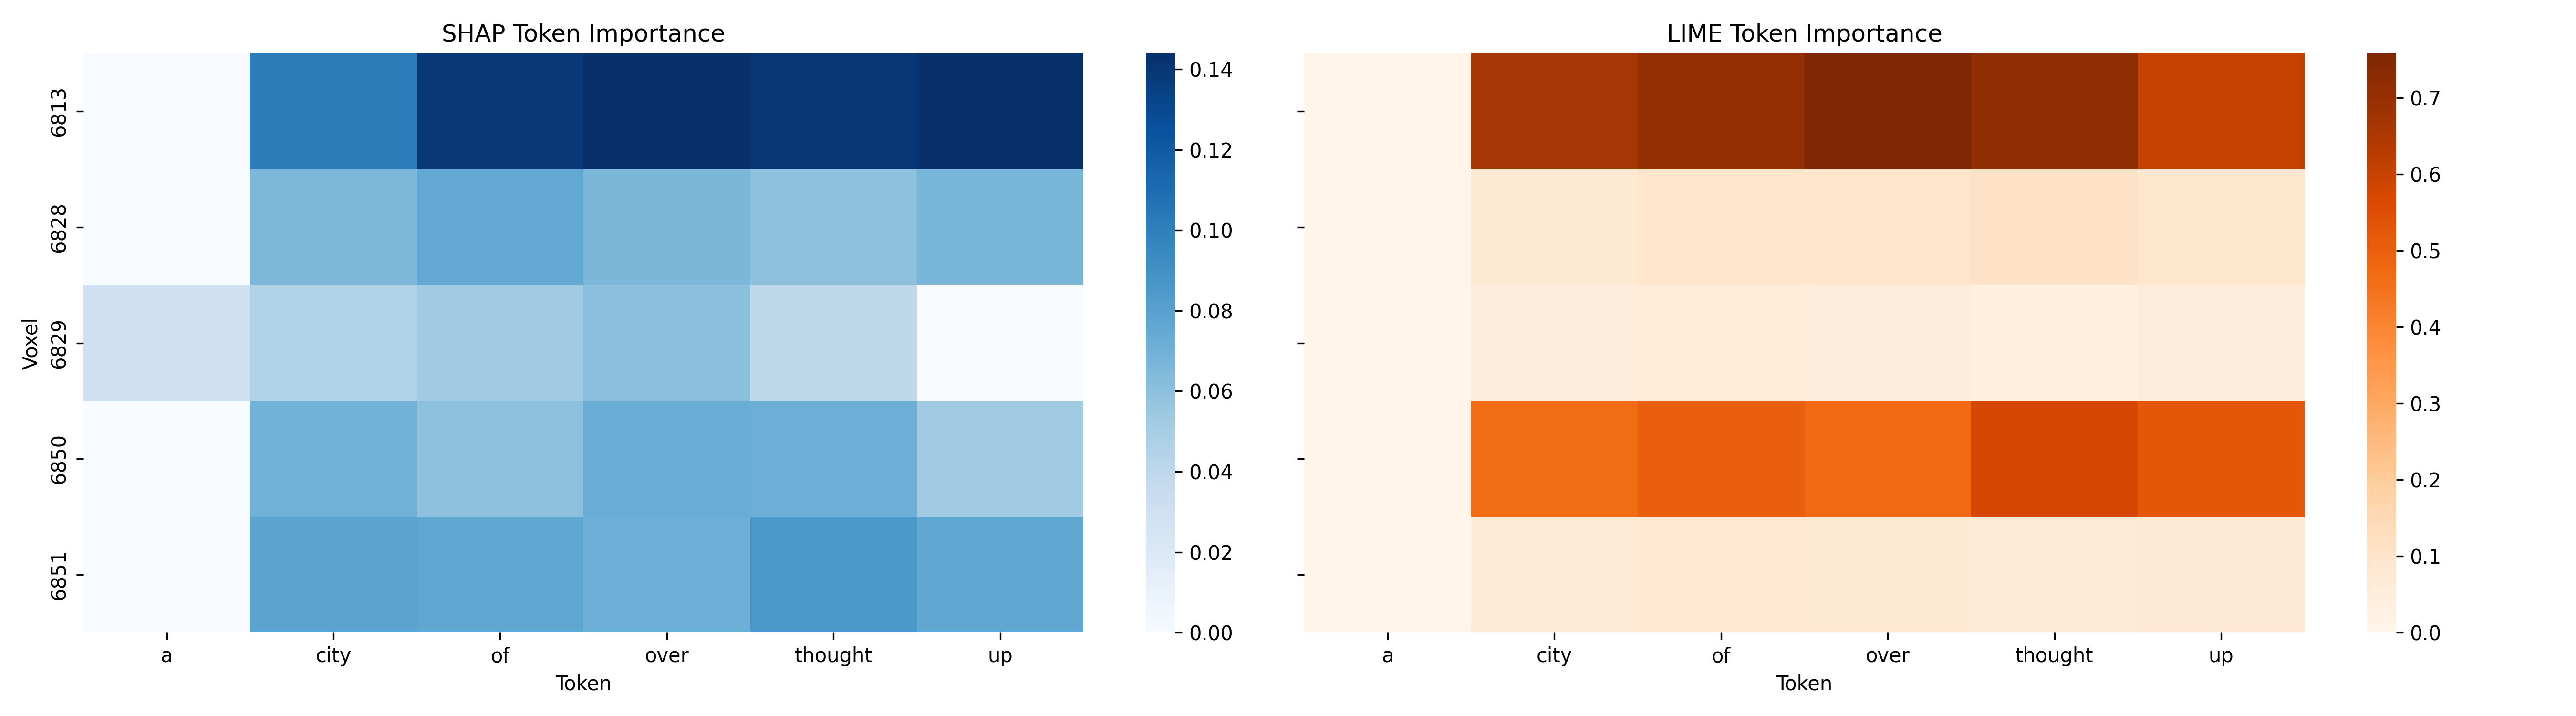
\includegraphics[width=\textwidth]{shap_lime_heatmap_quietfire.png}
\caption{Token importance heatmaps from SHAP and LIME for the top voxels in \textit{quietfire}.}
\label{fig:shap_lime_heatmap_quietfire}
\end{figure}

We examined the top tokens selected by SHAP and LIME for the five most predictive voxels (Table~\ref{tab:shap_lime_quietfire}). Both methods often picked out similar words—like “of,” “thought,” “city,” and “up”—which suggests that these tokens consistently influenced the model’s predictions. These words may have occurred frequently in the story or carried strong contextual meaning picked up by the model.

Looking at individual voxels, we noticed that some showed strong agreement between SHAP and LIME. For example, voxel 6813 gave high importance to “thought,” “over,” and “city” in both methods. Similarly, voxel 6828 highlighted “thought” and “city” consistently. But for voxel 6829, SHAP and LIME disagreed more: SHAP focused on “a” and “city,” while LIME emphasized “thought” and “over.” This might reflect differences in how each method captures signal or the role of local versus global context in different brain regions.

To help interpret these differences, we plotted heatmaps showing token importance scores for SHAP and LIME (Figure~\ref{fig:shap_lime_heatmap_quietfire}). The SHAP heatmap showed more even scores across multiple words, suggesting it reflects broader context over time. For example, voxels 6828 and 6851 had moderate importance across several tokens. In contrast, LIME showed sharper and more focused attribution: voxel 6813 had high scores only for “thought” and “up.” This shows that LIME tends to focus on a few strong signals, while SHAP spreads its importance across more context.

Unlike sloth, where SHAP and LIME often highlighted different types of words, the story quietfire showed greater alignment between the two methods. Tokens such as “thought,” “city,” and “of” were consistently important across multiple voxels and explanation methods, suggesting stable linguistic drivers. However, LIME remained more focused on a few dominant tokens per voxel, while SHAP distributed importance more broadly. These differences reaffirm the complementary nature of the two approaches—SHAP capturing integrative patterns over time and LIME isolating sharp, moment-specific drivers—while also highlighting how different narratives may evoke distinct patterns of brain-language correspondence.

\section{Academic Honesty}

\subsection{Statement}

We confirm that this report represents the collaborative work of our entire group. All analysis methods and procedures were jointly designed and executed. The text, figures, and research process have been documented transparently to ensure reproducibility. Any references to others’ work have been properly cited. Research integrity is fundamental to academic progress. While scholarship builds on prior knowledge, every study must uphold truthfulness, reliability, and originality. Irreproducible methods or unattributed work undermine trust and devalue collective scholarly efforts. As a team, we affirm our commitment to transparency, respect for intellectual contributions, and accountability for maintaining ethical standards. Each member has ensured that our work is original, properly cited, and advances understanding of brain-language modeling through honest collaboration.

\subsection{LLM Usage}

ChatGPT was used as a coding assistant for syntax validation and visualization enhancements, specifically for refining graph color schemes. All analytical decisions, model implementations, and evaluations were performed independently by the authors.

\bibliographystyle{alpha}
\bibliography{sample}

\end{document}